\documentclass[11pt,a4paper,english]{uvamath}
\usepackage[english]{babel}

\usepackage{amsmath, amsfonts, amssymb, a4wide, fancyhdr, lineno, graphicx, epsfig, soul, color, hyperref}
\usepackage[square, numbers]{natbib}

% Running line numbers:
\linenumbers
% Number only every 5:th line:
\modulolinenumbers[5]

%Nodig om een bibliography midden in het artikel te zetten, ipv aan het einde zoals eigenlijk gebruikelijk is
\renewcommand{\bibsection}{}

% TODO command
\newcommand{\todo}[1]{
    \hl{#1}
}

% The things that should be filled in by each group, depending on their situation, are written in a todo command, \todo{like this text}. All text in normal the normal font, is applicable for any group. However, everyone is free to adapt any text, and it is even suggested to look at all text critically and make changes if needed.

% Project specific commands
\author{Tom van Duist \& Kevin van den Bekerom}

\newcommand{\projectname}{\todo{Project Name}\ }


\newcommand{\aanpassen}[1]{ {\sethlcolor{green} \hl{#1}} }

\title{Reading assignment week 3}
%Variables
\newcommand{\TitelAbbr}{}
\newcommand{\Version}{0.1}



\what{}
\supervisors{}
\author{Tom van Duist}


\begin{document}

\maketitle
\clearpage


\chapter*{Reading assignment week 3}

\section*{4.1}

\subsection*{ \cite{req_en_book}}
Based on 
\begin{itemize}
	\item[\textbf{+}] 
	\item[\textbf{-}] 
\end{itemize}
\begin{figure}[h]
	\centering
	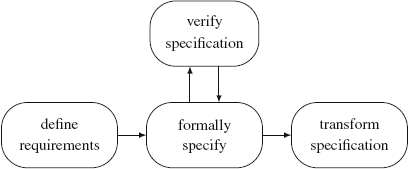
\includegraphics[width=0.75\linewidth]{Resources/4_transformational.png}
	\caption{The transformational process model.}
	\label{fig:transformational}
\end{figure} 

\clearpage
\subsection*{ \cite{req_en_book}}
Based on
\begin{itemize}
	\item[\textbf{+}] 
	\item[\textbf{-}] 
\end{itemize}
\begin{figure}[h]
	\centering
	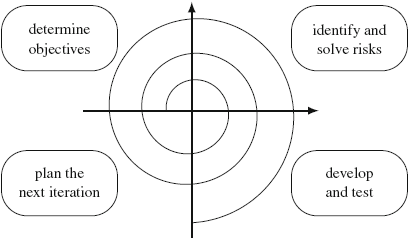
\includegraphics[width=0.75\linewidth]{Resources/4_spiral.png}
	\caption{The spirals model.}
	\label{fig:transformational}
\end{figure} 


\chapter{References}

\begin{thebibliography}{9}
	
	\bibitem{req_en_book}
	Joao M. Fernandes, Ricardo J. Machado, \\
	\emph{Requirements in Engineering Projects}
	
\end{thebibliography}


\appendix


\end{document}
